\section{SIR Model}
We introduce the SIR model as a motivating example and use-case for our implementation. It is a very well studied and understood compartment model from epidemiology \cite{kermack_contribution_1927} which allows to simulate the dynamics of an infectious disease like influenza, tuberculosis, chicken pox, rubella and measles \cite{enns_its_2010} spreading through a population. In this model, people in a population of size $N$ can be in either one of three states \textit{Susceptible}, \textit{Infected} or \textit{Recovered} at a particular time, where it is assumed that initially there is at least one infected person in the population. People interact \textit{on average} with a given rate of $\beta$ other people per time-unit and become infected with a given probability $\gamma$ when interacting with an infected person. When infected, a person recovers \textit{on average} after $\delta$ time-units and is then immune to further infections. An interaction between infected persons does not lead to re-infection, thus these interactions are ignored in this model. This definition gives rise to three compartments with the transitions as seen in Figure \ref{fig:sir_transitions}.

\begin{figure}
	\centering
	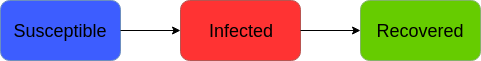
\includegraphics[width=.4\textwidth, angle=0]{./fig/SIR_transitions.png}
	\caption{States and transitions in the SIR compartment model.}
	\label{fig:sir_transitions}
\end{figure}

Before looking into how one can simulate this model in an agent-based approach we first explain how to formalize it using System Dynamics (SD) \cite{porter_industrial_1962}. In SD one models a system through differential equations, allowing to conveniently express continuous systems which change over time. The advantage of a SD solution is that one has an analytically tractable solution against which e.g. agent-based solutions can be validated. The problem is that the more complex a system, the more difficult it is to derive differential equations describing the global system, to a point where it simply becomes impossible. This is the strength of an agent-based approach over SD, which allows to model a system when only the constituting parts and their interactions are known but not the macro behaviour of the whole system. As will be shown later, the agent-based approach exhibits further benefits over SD.

The dynamics of the SIR model can be formalized in SD with the following equations:

TODO: there seems to be an unnerving space after the f letters, can we get rid of them?

\begin{align}
\frac{\mathrm d S}{\mathrm d t} &= -infectionRate \\ 
\frac{\mathrm d I}{\mathrm d t} &= infectionRate - recoveryRate \\ 
\frac{\mathrm d R}{\mathrm d t} &= recoveryRate 
\end{align}

\begin{align}
infectionRate &= \frac{I \beta S \gamma}{N} \\
recoveryRate &= \frac{I}{\delta} 
\end{align}

Solving these equations is done by integrating over time. In the SD terminology, the integrals are called \textit{Stocks} and the values over which is integrated over time are called \textit{Flows}. At $t = 0$ a single agent is infected because if there wouldn't be any infected agents, the system would immediately reach equilibrium - this is also the formal definition of the steady state of the system: as soon as $I(t) = 0$ the system won't change any more.

TODO: there seems to be an unnerving space after the f letters, can we get rid of them?

\begin{align}
S(t) &= N - I(0) + \int_0^t -infectionRate\, \mathrm{d}t \\
I(0) &= 1 \\
I(t) &= \int_0^t infectionRate - recoveryRate\, \mathrm{d}t \\
R(t) &= \int_0^t recoveryRate\, \mathrm{d}t
\end{align}

%There exist a large number of software packages which allow to conveniently express SD models using a visual approach like in Figure \ref{fig:sir_sd_stockflow_diagramm}.

%\begin{figure}
%	\centering
%	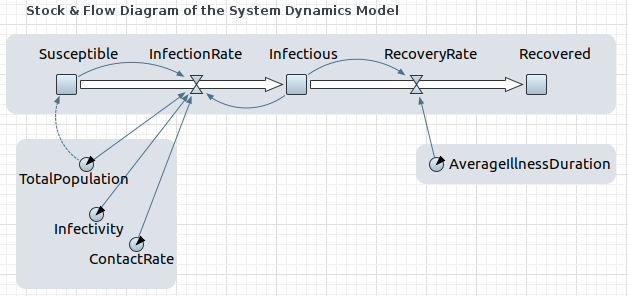
\includegraphics[width=.4\textwidth, angle=0]{./fig/diagrams/SIR_SD_STOCKFLOW_DIAGRAMM.png}
%	\caption{A visual representation of the SD stocks and flows of the SIR compartment model.} %Picture taken using AnyLogic Personal Learning Edition 8.1.0.
%	\label{fig:sir_sd_stockflow_diagramm}
%\end{figure}

Running the SD simulation over time results in the dynamics as shown in Figure \ref{fig:sir_sd_dynamics} with the given variables.

\begin{figure}
	\centering
	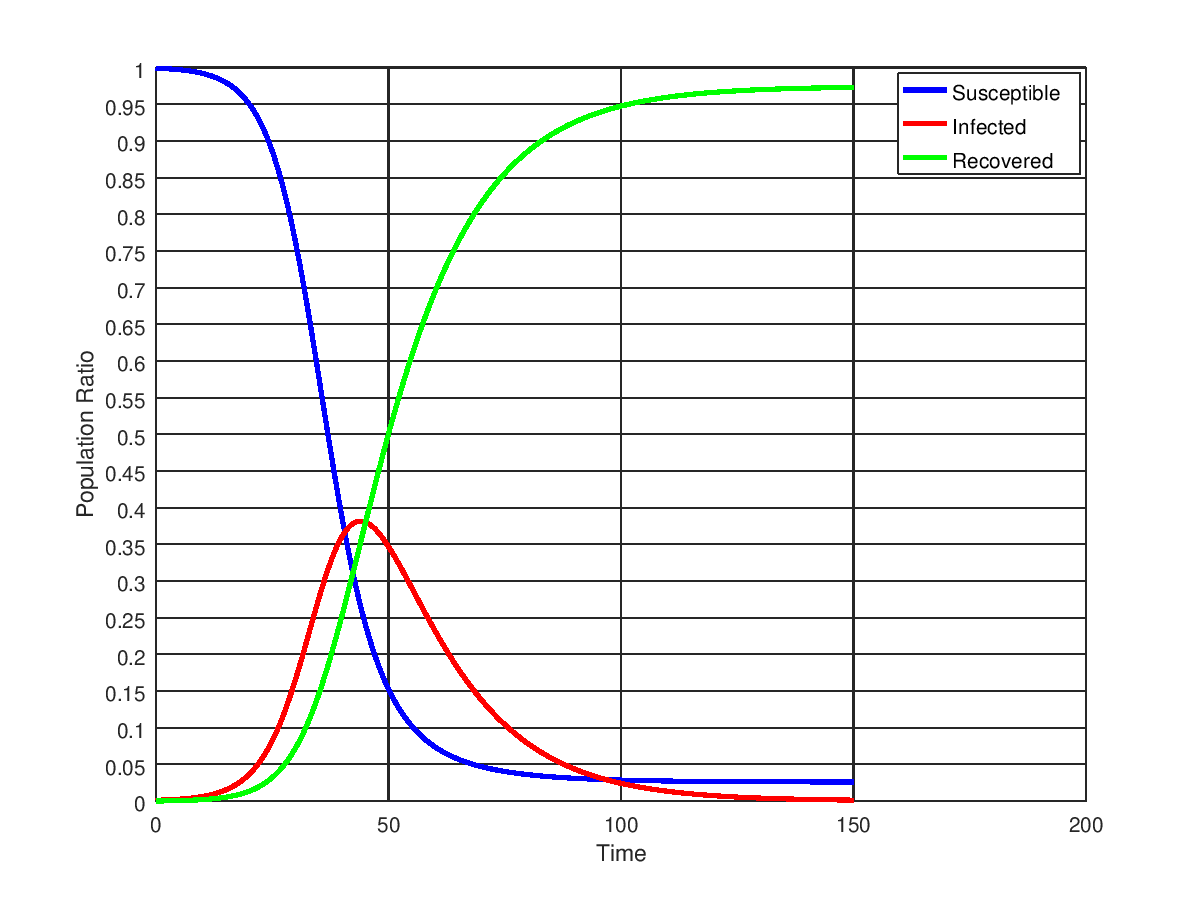
\includegraphics[width=.5\textwidth, angle=0]{./fig/SIR_SD_1000agents_150t_001dt.png}
	\caption{Dynamics of the SIR compartment model. Population Size $N$ = 1,000, contact rate $\beta =  \frac{1}{5}$, infection probability $\gamma = 0.05$, illness duration $\delta = 15$ with initially 1 infected agent. Simulation run for 150 time-steps.}
	\label{fig:sir_sd_dynamics}
\end{figure}
